\begin{mydefs}
	Dans un triangle :
	\begin{itemize}
		\item La \hspace*{4cm} d'un coté est la droite perpendiculaire à ce coté et passant par son milieu.
		
		\item Une droite qui passe par un sommet et est perpendiculaire à la droite qui porte le coté opposé est une \hspace*{3cm} du triangle. 
	\end{itemize}
\end{mydefs}

\begin{myexs}
	\begin{multicols}{2}
		Dans la figure ci-contre :
		
		\begin{itemize}
			\item \hspace*{1cm} est la hauteur issue de \hspace*{1cm}, $H$ est le pied de cette hauteur;
			\item \hspace*{1cm} est la hauteur issue de \hspace*{1cm}, $E$ est le pied de cette hauteur;
			\item \hspace*{1cm} est la médiatrice du coté 
		\end{itemize}
		\begin{center}
			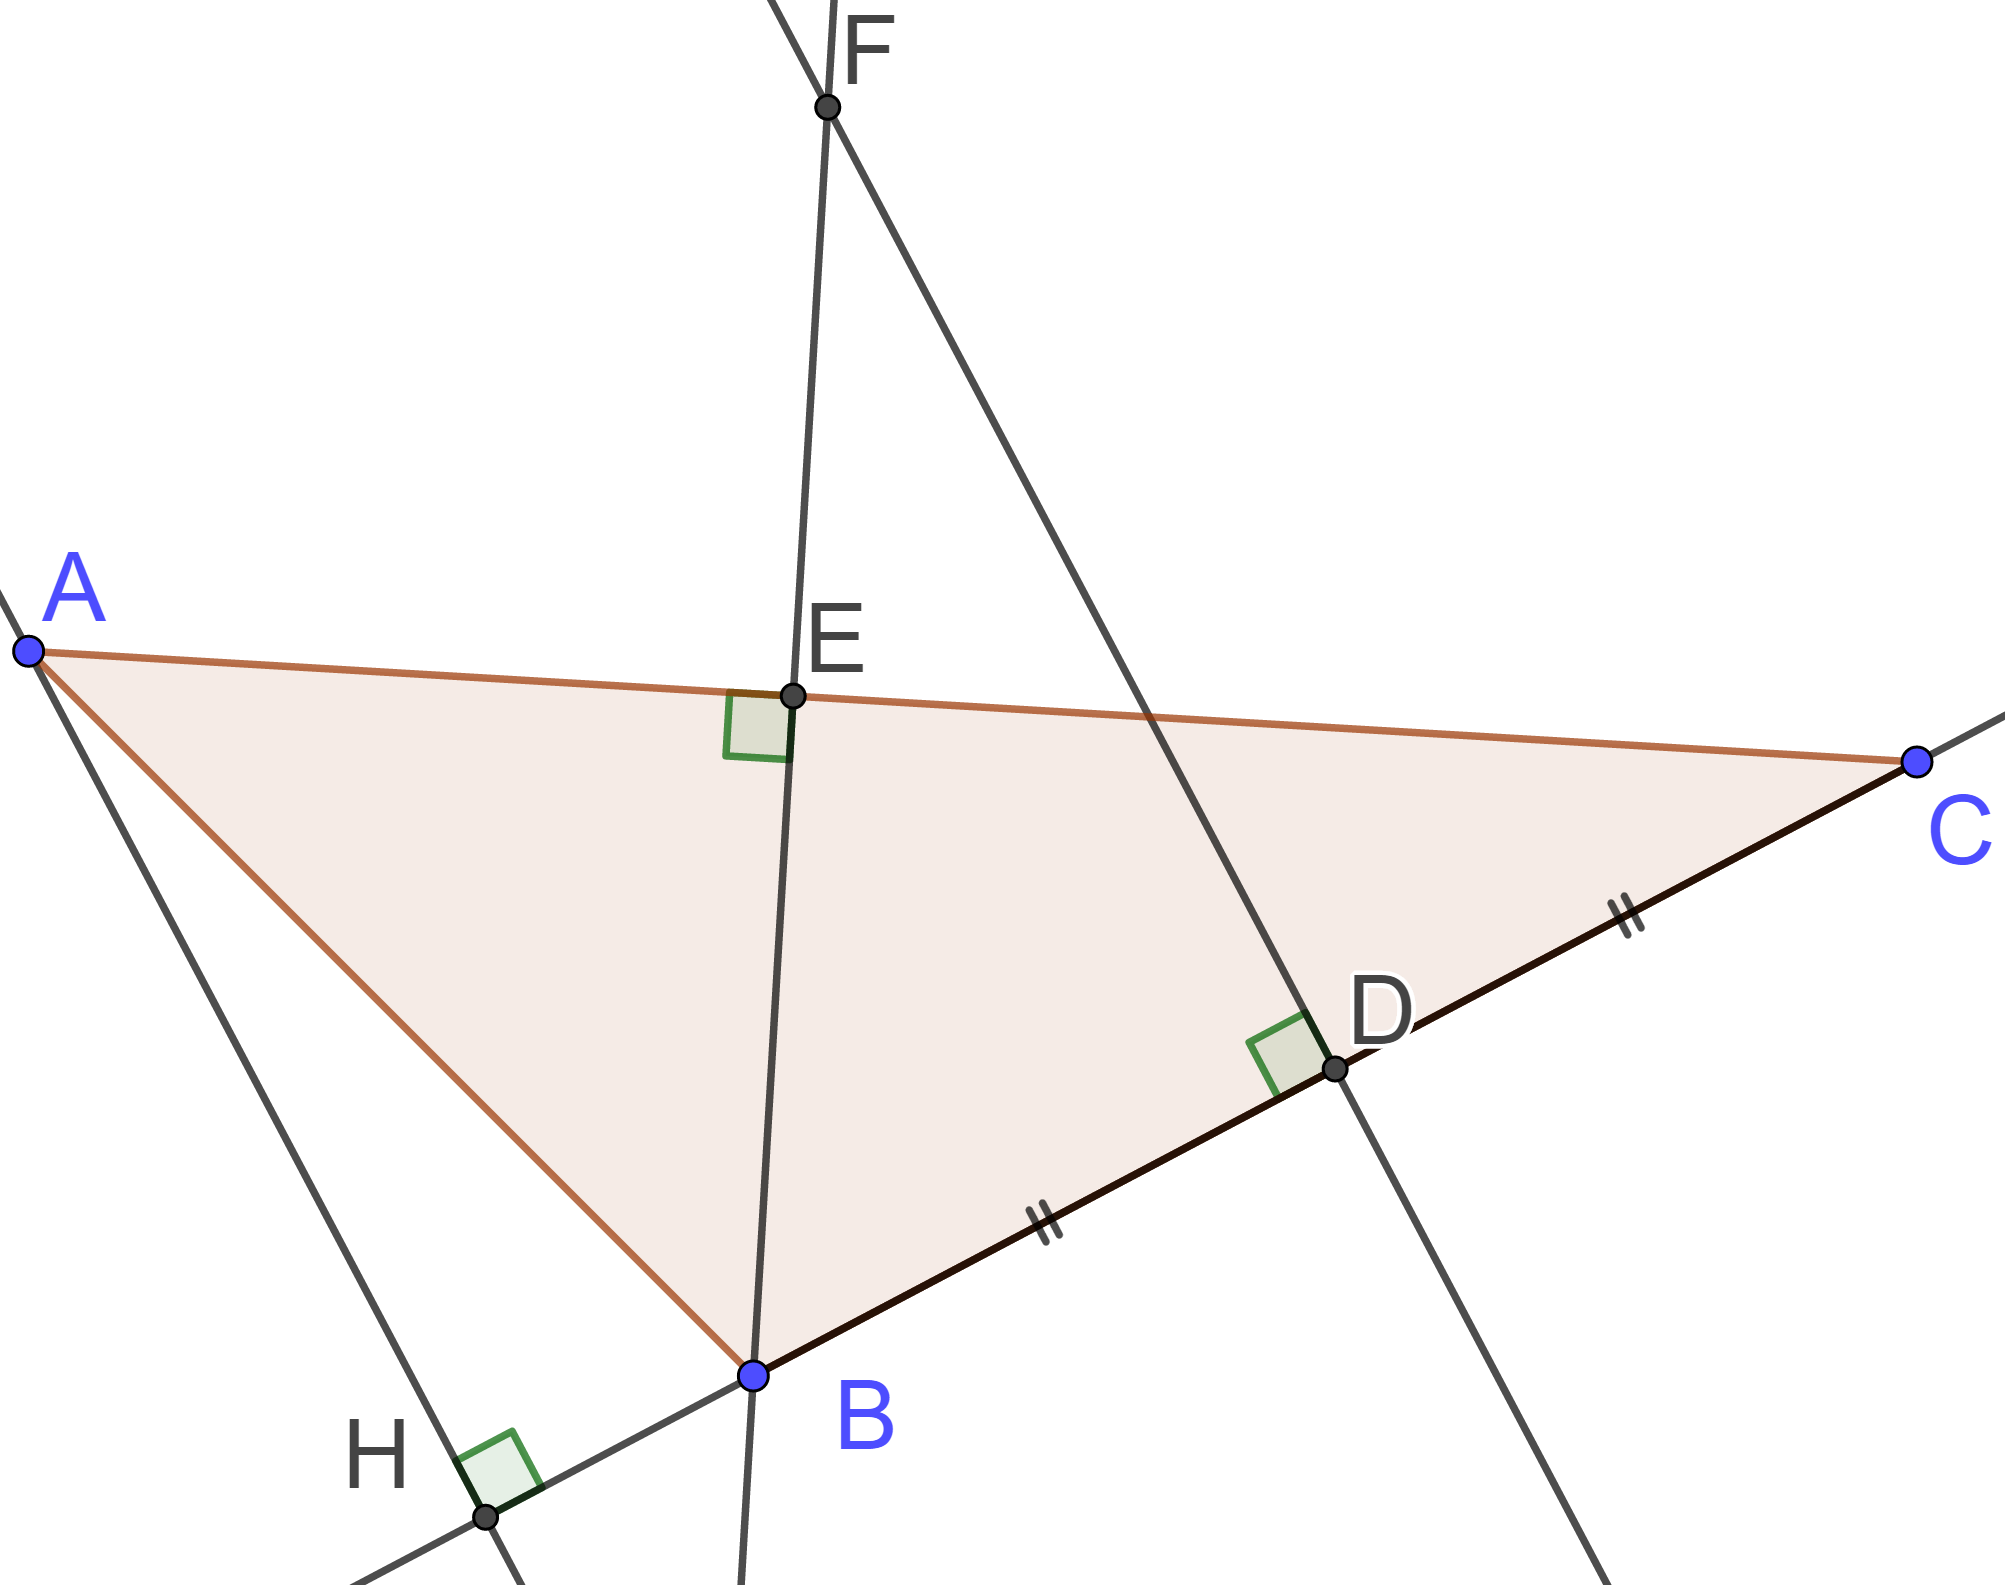
\includegraphics[scale=0.15]{droites}
		\end{center}
	\end{multicols}
\end{myexs}